\documentclass[a4paper]{article}
\usepackage{listings}
\usepackage{qtree}
\usepackage{xcolor}
\usepackage{forest}
\usepackage{multicol}
\setlength{\columnsep}{3cm}
\usepackage{parskip}
\usepackage{changepage}
\usepackage[T1]{fontenc}
\usepackage{amsmath}
\usepackage{hyperref}
\usepackage{listings}
\usepackage{amsthm}
\usepackage{amssymb}
\usepackage{float}
\usepackage[utf8]{inputenc}
\usepackage{graphicx}
\usepackage[italian]{babel}
\usepackage{thmtools}
\begin{document}
\addtolength{\topmargin}{-100pt}
\addtolength{\textheight}{160pt}


\author{Lorenzo Dentis, lorenzo.dentis@edu.unito.it}
\title{Produttori e consumatori in PA e Nusmv}
\maketitle
\section{Process Algebra}
\subsection{1 produttore, 1 consumatore, buffer a N posizioni}
\label{SEC:PA_1}
Il sistema è organizzato come segue:
\begin{flalign*}
	&SYS = (Prod || Cons || (Buffer)) /_{\{put,get,passa\} }&&\\
	&Prod=think.produce.\overline{PUT}.Prod&&\\
	&Cons=think.produce.\overline{GET}.Cons&&\\
	&\textit{funzioni di Relabeling:}&&\\
	&f_E\bigg[\begin{aligned} &put \rightarrow put\\ &get \rightarrow passa_1 \end{aligned}\bigg] &&\\
	&f_F\bigg[\begin{aligned} &put \rightarrow \overline{passa}_{n-1}\\ &get \rightarrow passa_{n} \end{aligned}\bigg] \; \forall n \in [1,N] &&\\
	&f_E\bigg[\begin{aligned} &put \rightarrow put\\ &get \rightarrow \overline{passa}_{n} \end{aligned}\bigg] &&\\
	&Buffer = \underbrace{E_{[f_E]}|| ... || E_{[f_M]} || ... || E_{[f_F]}}_{N \text{ volte}}&&\\
	&E=PUT.F&&\\
	&F=GET.E&&
\end{flalign*}
Le operazioni $put,get$ sono inserite in una restrizione, in modo che sia possibile inserire e rimuovere oggetti dal buffer solamente tramite $\tau$-operazioni che coinvolgono una "cella" del buffer ed uno tra il consuamtore ed il produttore.\\
Non è possibile indicare un buffer a $N$ posizioni in maniera generica quindi ho costruito il buffer come una composizione di $N$ buffer ad 1 posizione, dato che l'esercizio richiede che non il buffer sia un unico oggetto e non sia possibile inserire elementi in differenti "celle" di questo ho definito tre funzioni di relabeling ed una nuova operazione $passa_n$ anche essa inserita nella restrizione.
\begin{itemize}
	\item $f_E$: operazione effettuabile solo da una cella del buffer, è l'unica cella che può effettuare operazioni di $put$, obbligando il produttore ad inserire dati solo in quella cella.
	\item $f_F$: operazione effettuabile solo da una cella del buffer, è l'unica cella che può effettuare operazioni di $get$, obbligando il consumatore a prelevare dati solo da quella cella.
	\item $f_M$: questa funzione di relabeling permette alle celle del buffer differenti da quella iniziale e quella finale di passare il dato verso il fondo del buffer.
\end{itemize}
\begin{figure*}[!ht]
\centering
\makebox[\textwidth][c]{
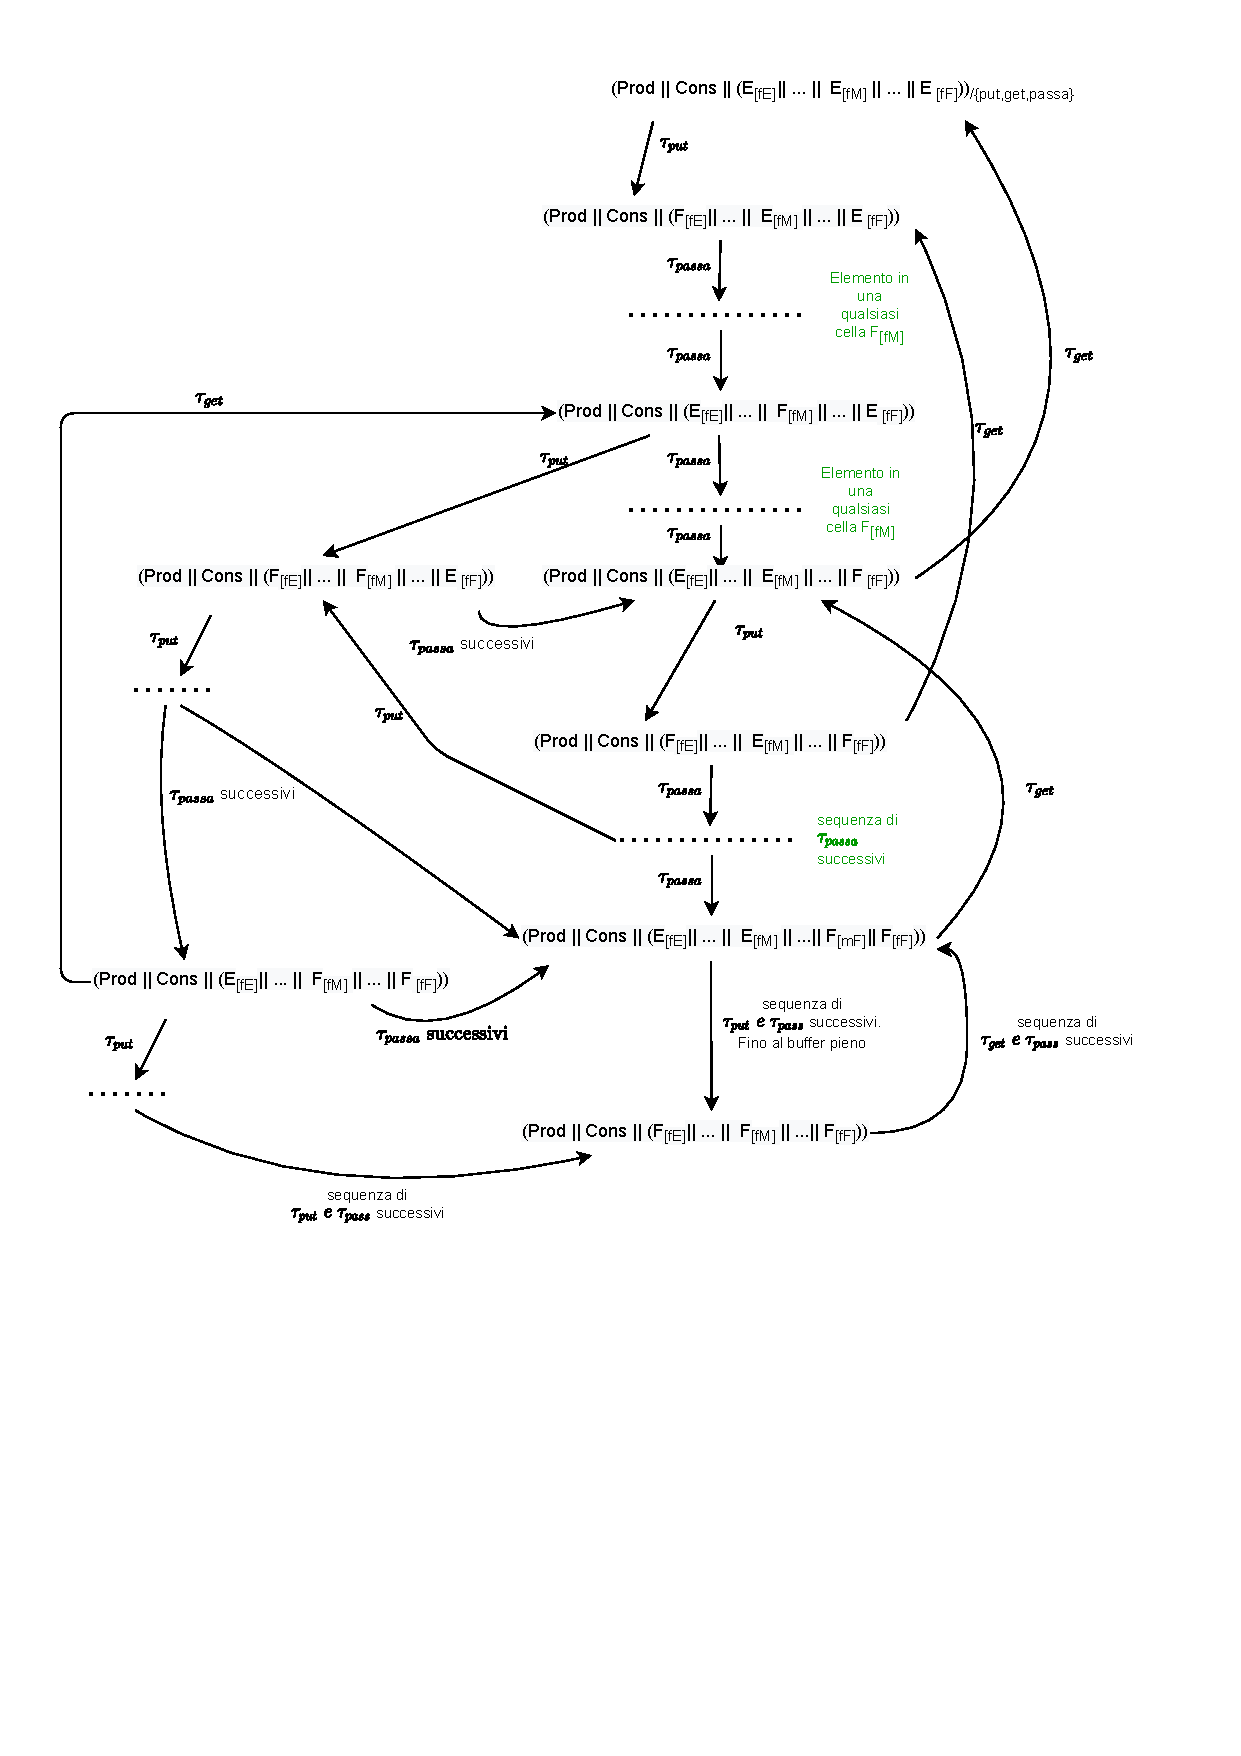
\includegraphics[width=1.2\textwidth]{./PA/setting1}}
\caption{Setting1} \label{FIG:PA1_DG}
\end{figure*}
Lo scopo principale di questo \textit{derivation graph} è mostrare il funzionamento del buffer a N posizioni, l'operazione di $put$ può essere effettuata solo sulla prima cella del buffer e l'operazione di $get$ solo sull'ultima.
Il buffer può liberamente compiere operazioni interne $passa_n$ che causano un "effetto cascata".
Quando un elemento viene inserito nella prima cella questa lo passa alla seconda, che lo passa alla terza e via così fino all'ultima, dalla quale può essere rimosso.\\
Le operazioni interne al buffer sono state rappresentate informalmente con il termine $\tau_{passa[n]}$ per distinguerle chiaramente dalle operazioni svolte dal produttore e dal consumatore, rispettivamente $\tau_{get}$ e $\tau_{put}$.\\
Notiamo che le operazioni \textit{passa} non sono obbligate, un elemento potrebbe rimanere in una cella differente dall'ultima.
Questa proprietà ha una conseguenza, un produttore potrebbe voler effettuare una $put$ quando gli elementi non sono per forza accodati verso il fondo, e ciò gli sarebbe permesso in quanto il la prima cella del buffer è libera.
Tale operazione rende impossibile la rappresentazione del \textit{derivation graph} di un buffer a $N$ posizioni dato che genera infinite possibili $\tau_{get}$ operazioni, tutte le possibili interfogliazioni tra le operazioni svolte dal produttore e le operazioni del buffer sono infinite.
É interessante notare come questo problema non si pone nel caso opposto, se un consumatore vuole estrarre un elemente deve attendere che il buffer abbia concluso tutte le sue operazioni interne, altrimenti non vi è alcun elemento nell' ultima cella.
Nelle implementazioni successive assumeremo per semplicità che il buffer sia a 3 posizioni per ottenere un numero di $\tau_{passa}$ finito pur continuando a mostrare la situazione in cui un elemento viene inserito o rimosso dal buffer prima che le operazioni di "spostamento" siano state concluse.


\subsection{1 produttore, 2 consumatori, buffer a N posizioni}
\label{SEC:PA2}
Il sistema in questo caso è molto simile al sitema del caso precedente, l'unica aggiunta è la concatenazione di un ulteriore Cons.\\
\begin{flalign*}
	&SYS = (Prod || Cons || Cons || (Buffer)) /_{\{put,get,passa\} }&&\\
	&Prod=think.produce.\overline{PUT}.Prod&&\\
	&Cons=think.produce.\overline{GET}.Cons&&\\
	&\textit{funzioni di Relabeling:}&&\\
	&f_E\bigg[\begin{aligned} &put \rightarrow put\\ &get \rightarrow passa_1 \end{aligned}\bigg] &&\\
	&f_F\bigg[\begin{aligned} &put \rightarrow \overline{passa}_{n-1}\\ &get \rightarrow passa_{n} \end{aligned}\bigg] \; \forall n \in [1,N] &&\\
	&f_E\bigg[\begin{aligned} &put \rightarrow put\\ &get \rightarrow \overline{passa}_{n} \end{aligned}\bigg] &&\\
	&Buffer = \underbrace{E_{[f_E]}|| ... || E_{[f_M]} || ... || E_{[f_F]}}_{N \text{ volte}}&&\\
	&E=PUT.F&&\\
	&F=GET.E&&
\end{flalign*}
\begin{figure*}[!ht]
\centering
\makebox[\textwidth][c]{
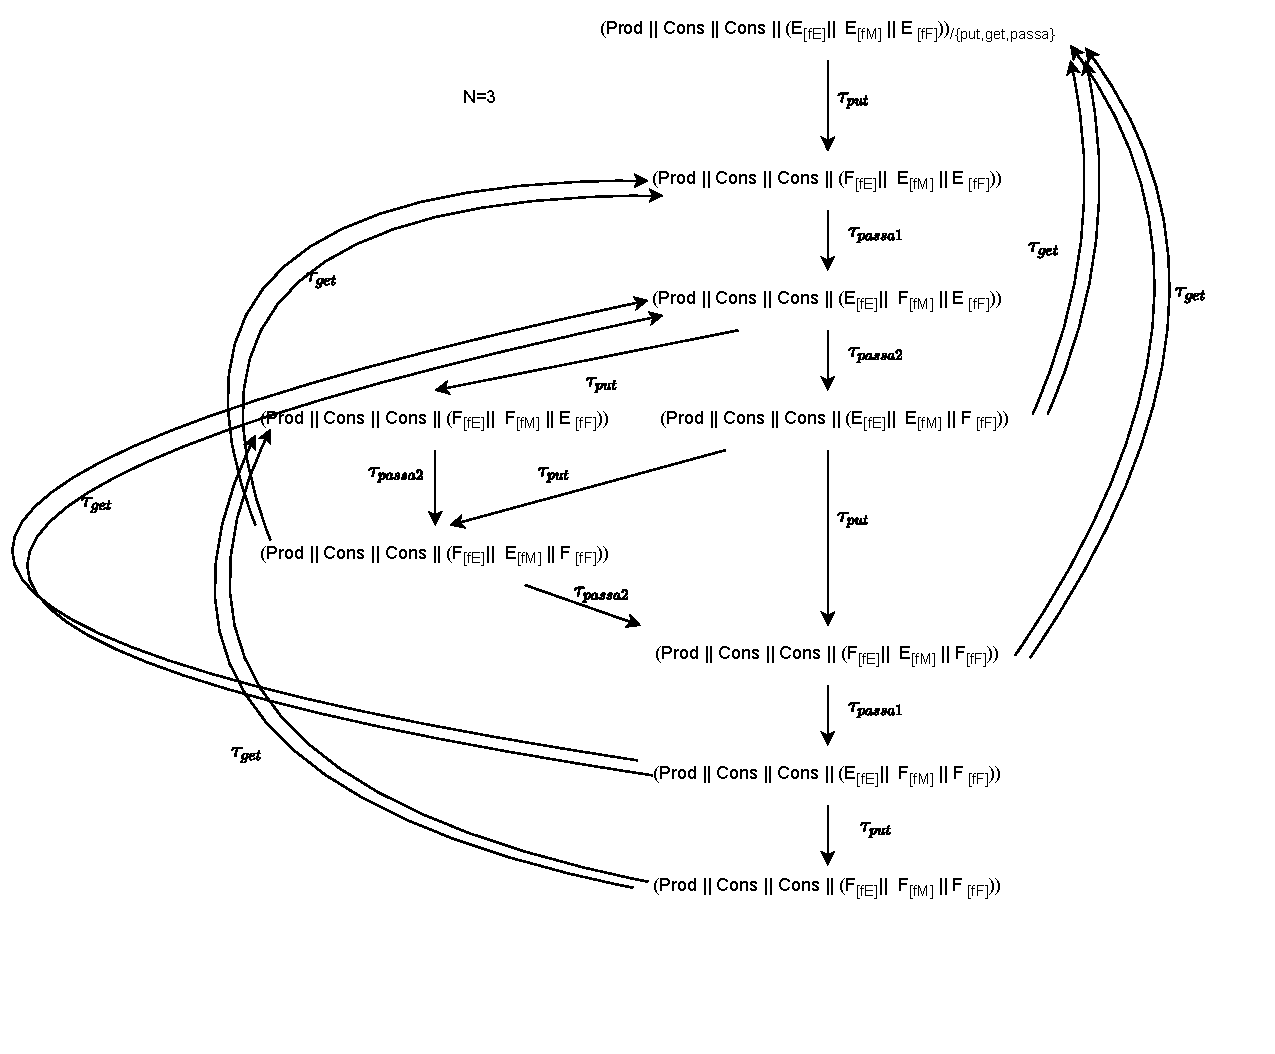
\includegraphics[width=1.2\textwidth]{./PA/setting2}}
\caption{Setting2} \label{FIG:PA2_DG}
\end{figure*}
In questo \textit{derivation graph} si è considerata solo la situazione in cui il buffer è limitato a 3 posizioni, dato che tale assunto semplifica la lettura ed in ogni caso la situazione con buffer ad N posizioni è stata già discussa nella sezione precendente (sezione \ref{SEC:PA_1}).
La presenza di un ulteriore consumatore non modifica molto il grafo, infatti aggiunge solo ad ogni stato (escluso lo stato con il buffer completamente vuoto) la possibilità di effettuare due distinte operazioni $\tau_{get}$, una per ogni \textit{Consumer}.
Entrambe le operazioni $\tau_{get}$, nonostante siano svolte da due \textit{Consumer} differenti, conducono a due stati indistinguibili che ho quindi accorpato in uno stato solo.
\subsection{P produttori, C consumatori, buffer a N posizioni}
Questo caso comporta lo stesso problema di implementazione (raffiguare un buffer a N posizioni), anche per i \textit{Produttori} ed i \textit{consumatori}.
\begin{flalign*}
	&SYS = (\underbrace{Prod || ... ||Prod}_{P \textit{ volte}} || \underbrace{Cons || ... ||Cons}_{C \textit{ volte}} || (Buffer)) /_{\{put,get,passa\} }&&\\
	&Prod=think.produce.\overline{PUT}.Prod&&\\
	&Cons=think.produce.\overline{GET}.Cons&&\\
	&\textit{funzioni di Relabeling:}&&\\
	&f_E\bigg[\begin{aligned} &put \rightarrow put\\ &get \rightarrow passa_1 \end{aligned}\bigg] &&\\
	&f_F\bigg[\begin{aligned} &put \rightarrow \overline{passa}_{n-1}\\ &get \rightarrow passa_{n} \end{aligned}\bigg] \; \forall n \in [1,N] &&\\
	&f_E\bigg[\begin{aligned} &put \rightarrow put\\ &get \rightarrow \overline{passa}_{n} \end{aligned}\bigg] &&\\
	&Buffer = \underbrace{E_{[f_E]}|| ... || E_{[f_M]} || ... || E_{[f_F]}}_{N \text{ volte}}&&\\
	&E=PUT.F&&\\
	&F=GET.E&&
\end{flalign*}
Fortunatamente (come nel caso di sezione \ref{SEC:PA2}) tutte le operazioni svolte dai molteplici \textit{Produttori \textit{e} Consumatori} conducono a stati tra loro indistinguibili.\\
L'unica differenza rilevante sta nel numero di $\tau$-operazioni eseguibili, in figura rappresentate tramite frecce con righe composte da puntini.Da ogni stato avente "la prima" cella del buffer vuota sarà possibile effettuare $P$ operazioni $\tau_{put}$ e da ogni stato avente "l' ultima" cella piena è sarà possibile effettuare $C$ operazioni $\tau_{get}$.\\
Come nel caso \ref{SEC:PA2} da ogni stato avente almeno un elemento nel buffer è possibile effettuare $N - elements - 1$ $\tau_{passa}$-transizioni, ove $elements$ è il numero di celle del buffer occupate.\\
\begin{figure*}[!ht]
\centering
\makebox[\textwidth][c]{
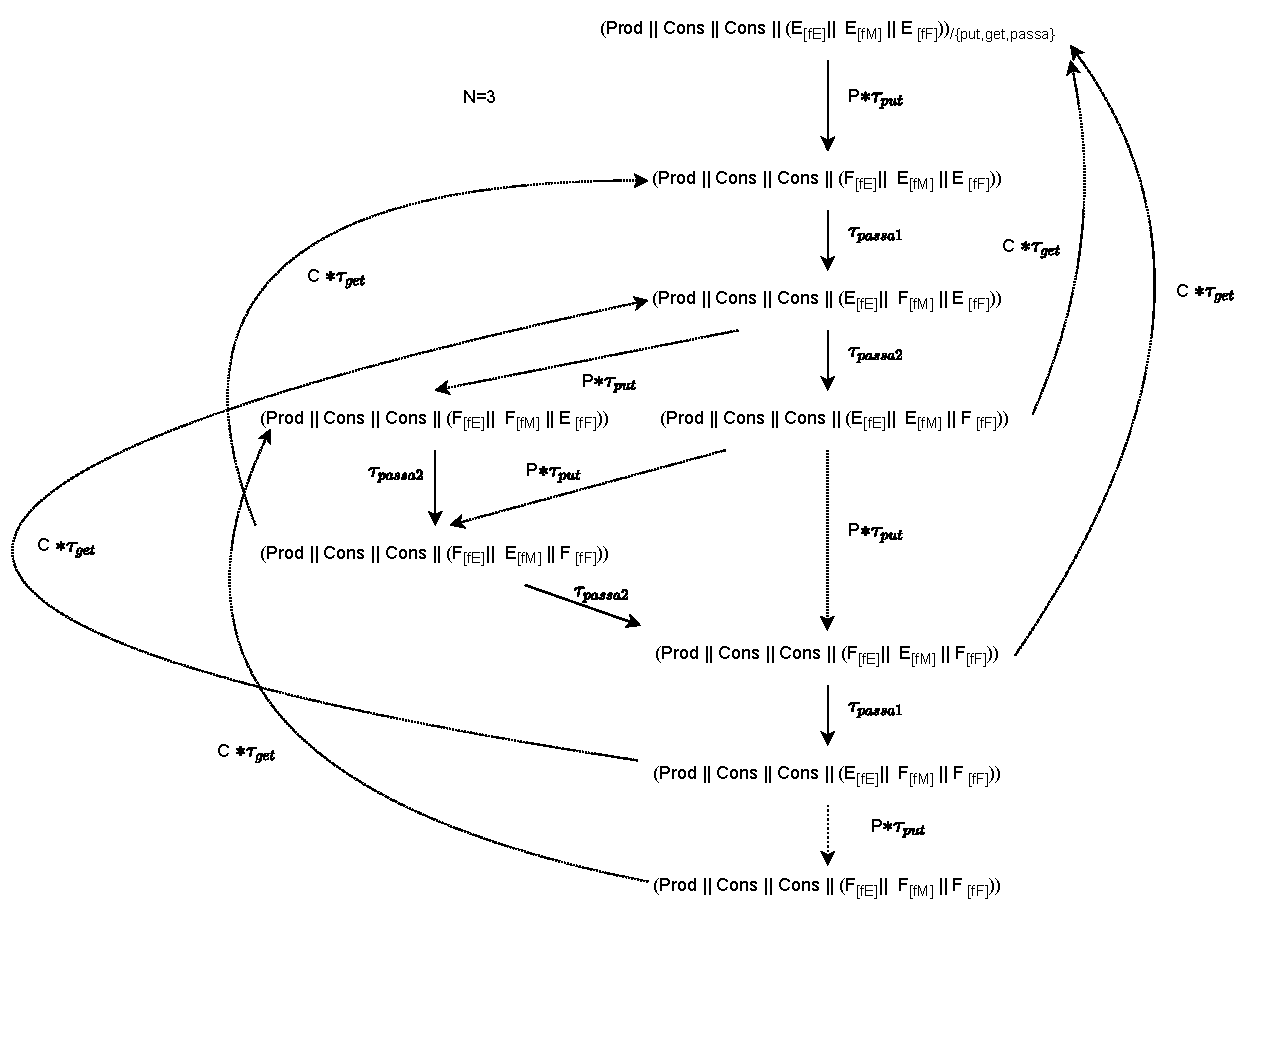
\includegraphics[width=1.2\textwidth]{./PA/setting3}}
\caption{Setting3} \label{FIG:PA3_DG}
\end{figure*}
\newpage

\section{NuSMV}
%todo: fare reachable_state -v e commentare la dimensione rispetto alla reti di petri. sarà minore perchè alle reti ho eliminato un posto "inutile". sengarlo o modificare le reti di petri.
\subsection{1 produttore, 1 consumatore, buffer a N posizioni}
\lstinputlisting[numbers=left,firstnumber=1,stepnumber=1,basicstyle=\small]{nusmv/consegnare/es_3_setting_1.smv}
In questo programma il buffer è identificato da una variabile intera che può assumere valori compresi tra 0 e 3, volendo incrementare la dimensione del buffer bisogna modificare il valore 3 inserendo il valore desiderato.
Non c'è quindi la possibilità di impostare il valore del buffer in maniera interattiva ma quantomeno lo si può gestire parametricamente.\\
I due processi ricevono come parametro il buffer ed hanno una semplice implementazione dei passaggi di stato: l'unica limitazione inserita è nell'uscita dallo stato \texttt{place}/\texttt{take} che corrisponde all'operazione di aggiunta/rimozione di un elemento dal buffer.\\
Il \textit{Consumer} non può effettuare l'operazione \textit{get} se il buffer è vuoto (riga 36), così come il \textit{producer} non puà effettuare una \textit{put} se il buffer è già pieno (riga 19).

Invece il buffer viene incrementato o decrementato solo quando un processo effettua una operazione su di esso (righe 24 e 41), la sintassi di \textit{NuSMV} obbliga l'inserimento di una clausola che impedisca al buffer di superare il valore 3 o scendere sotto il valore 0.
\newpage
\subsection{1 produttore, 2 consumatori, buffer a N posizioni}
\lstinputlisting{nusmv/consegnare/es_3_setting_2.smv}
Come nelle altre implementazioni il setting 2 è praticamente identico al setting 1. In questo caso la differenza sta nell'introduzione di una nuova variabile Cons2, istanza di \texttt{process consumer}.
Si può però notare che non è necessaria alcuna forma di mutua esclusione esplicita in quanto le operazioni di \texttt{place} e \texttt{take} sono intese come operazioni atomiche.
\subsection{P produttori, C consumatori, buffer a N posizioni}
Questa implementazione non è possibile, in quanto \emph{NuSMV} non permette la creazione di vettori di processi, l'unico modo di generare P produttori e C consumatori è quindi scrivere P variabili di tipo \texttt{process prod} e C variabili di tipo \texttt{process cons}.
\end{document}
